\setcounter{section}{1}
\appendix
\clearpage{\renewcommand{\appendixname}{Anexo}

\chapter{Interfaz de usuario del sistema SECPROIT}

\section{Limtaciones del SECPROIT}
\begin{figure}[H]
\centering
 \frame{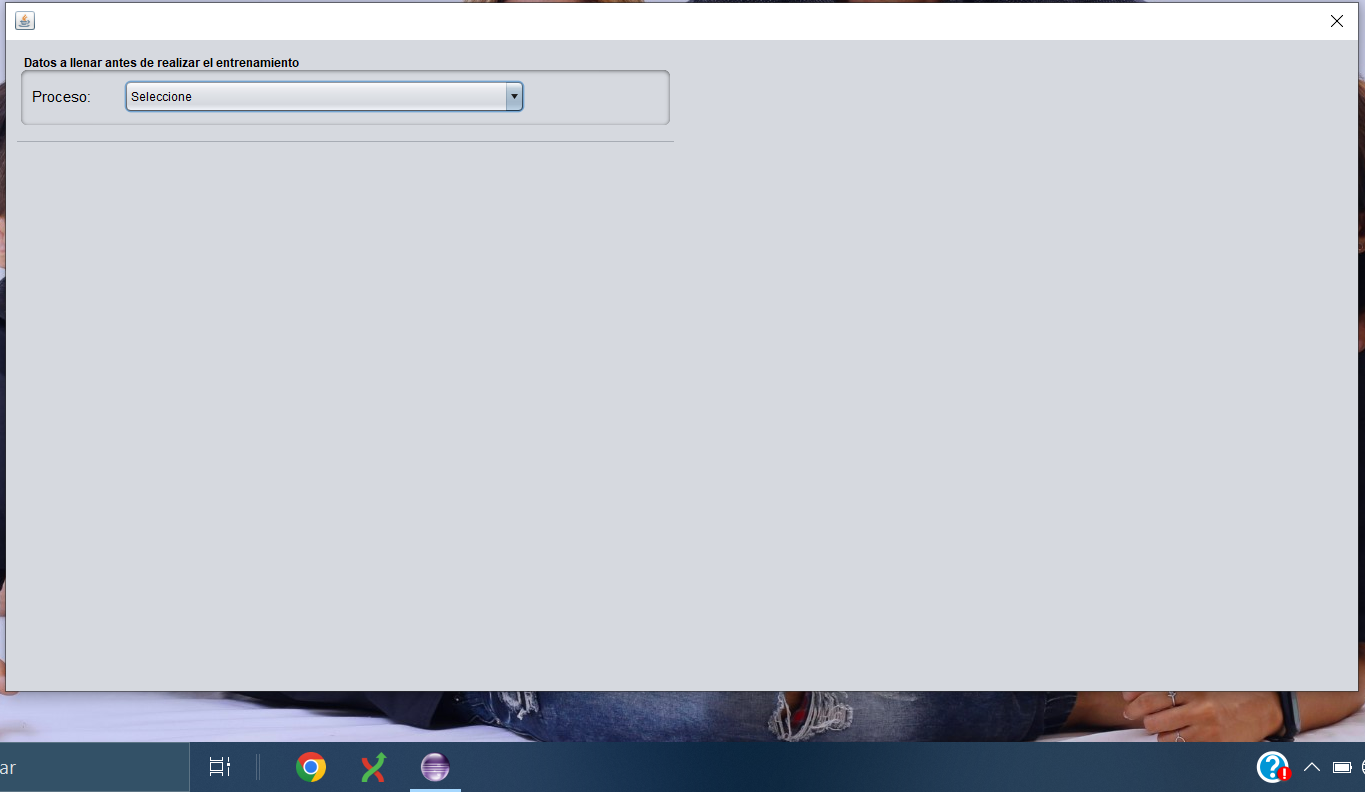
\includegraphics[width=0.9\linewidth]{imagen/anexos/sinicono.png}}
 \caption{No presenta icono de sistema}
 \label{fig:noIcono} 
\end{figure}

\begin{figure}[H]
\centering
 \frame{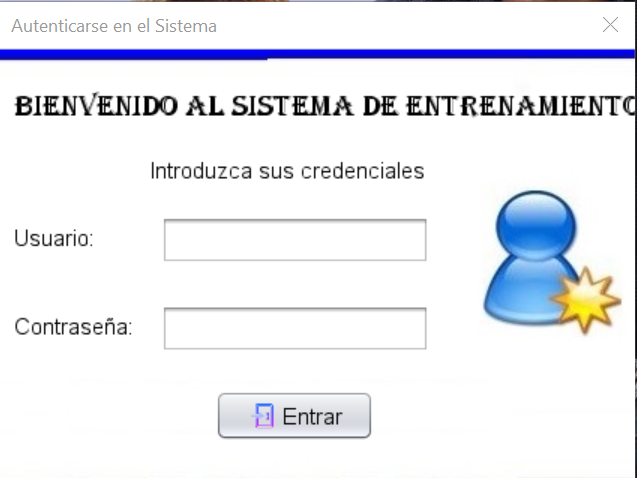
\includegraphics[width=0.6\linewidth]{imagen/anexos/titulo.png}}
 \caption{Aparecen títulos cortados por la vista}
 \label{fig:titulo} 
\end{figure}

\begin{figure}[H]
\centering
 \frame{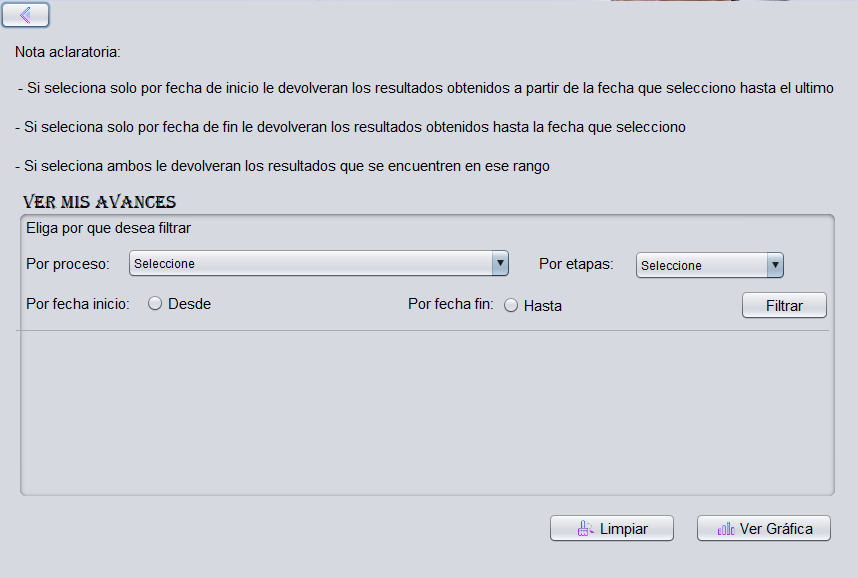
\includegraphics[width=0.9\linewidth]{imagen/anexos/bordes.png}}
 \caption{Visuales sin bordes}
 \label{fig:bordes} 
\end{figure}

\begin{figure}[H]
\centering
 \frame{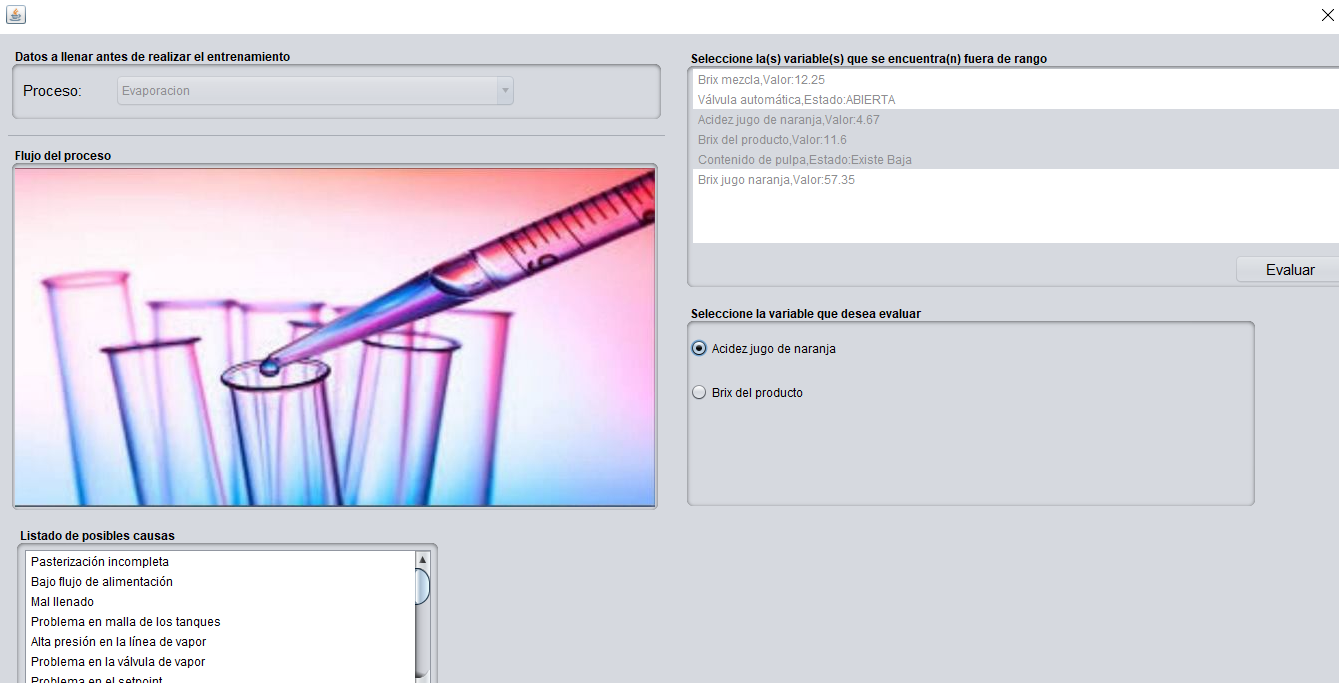
\includegraphics[width=0.9\linewidth]{imagen/anexos/tamanno.png}}
 \caption{El contenido se muestra a medias}
 \label{fig:tamano} 
\end{figure}

\begin{figure}[H]
\centering
 \frame{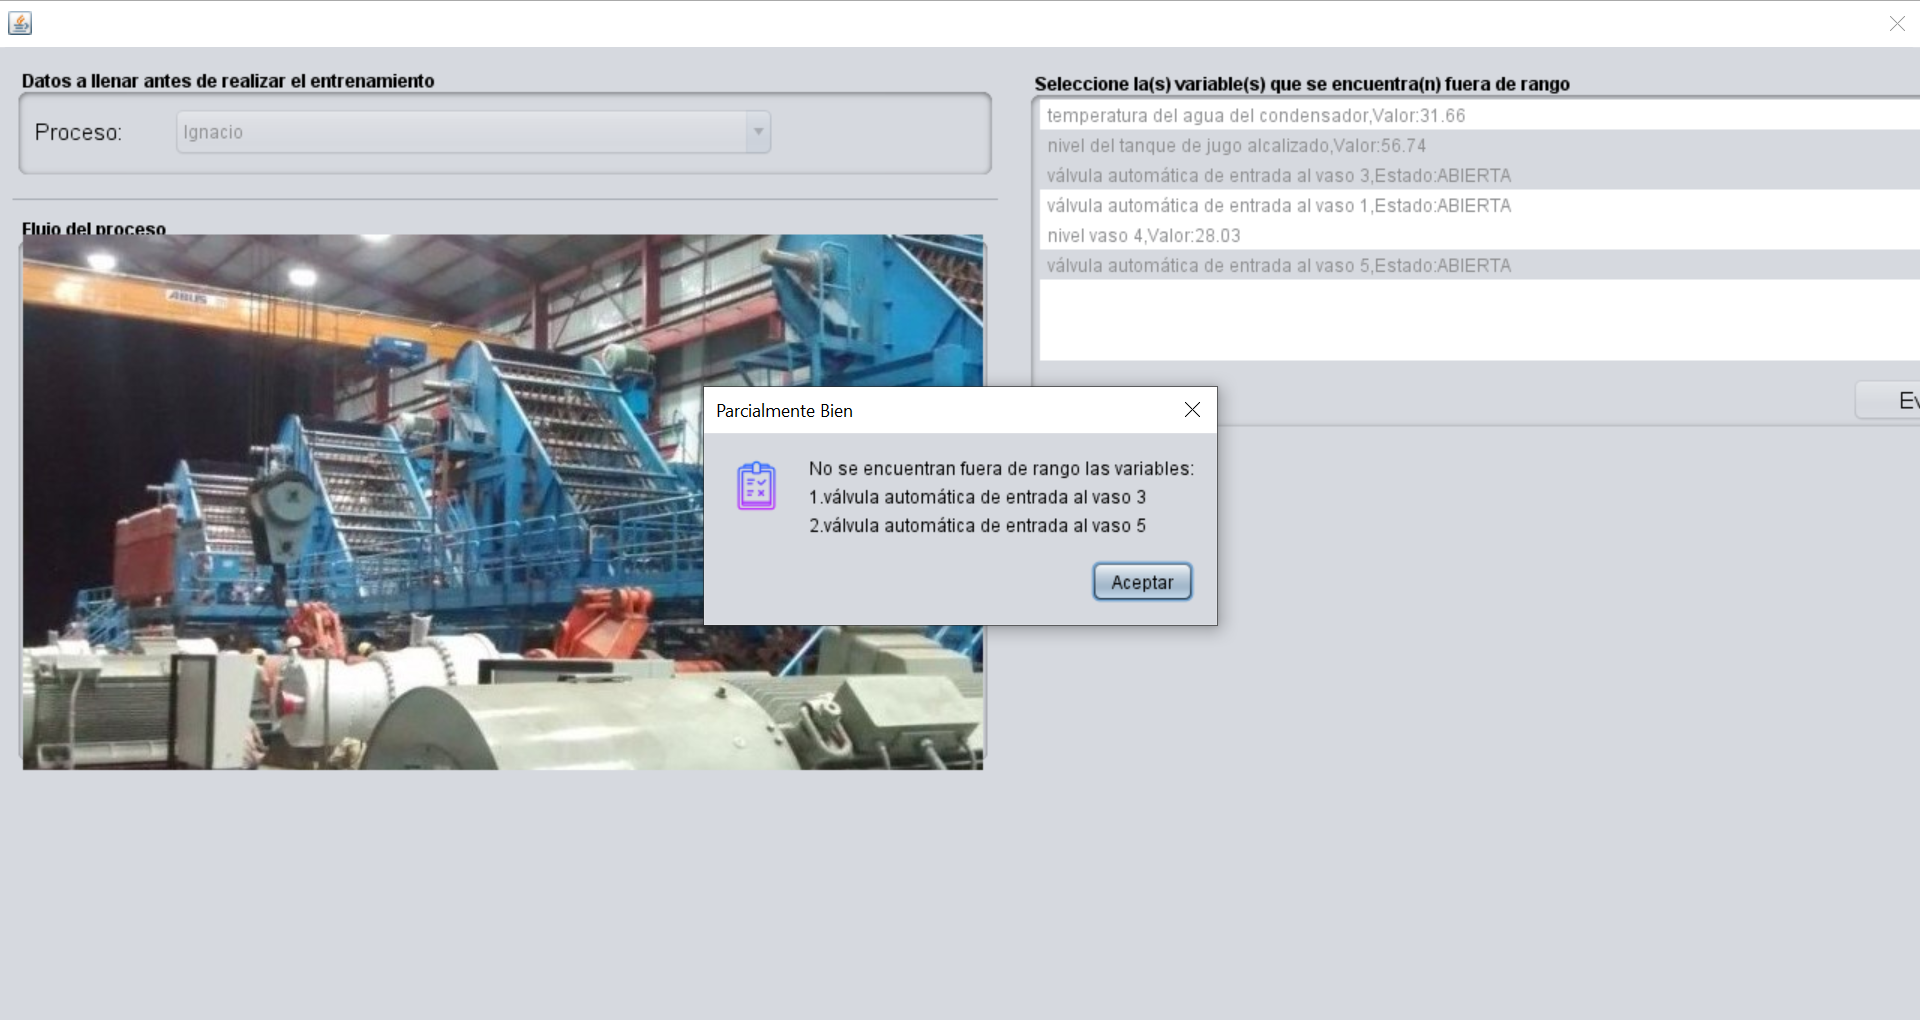
\includegraphics[width=0.9\linewidth]{imagen/anexos/innecesario.png}}
 \caption{Espacios en blanco innecesarios}
 \label{fig:inn} 
\end{figure}

\chapter{Interfaz de usuario del nuevo sistema de capacitación}

\section{Gestión de usuarios}
\begin{figure}[H]
\centering
 \frame{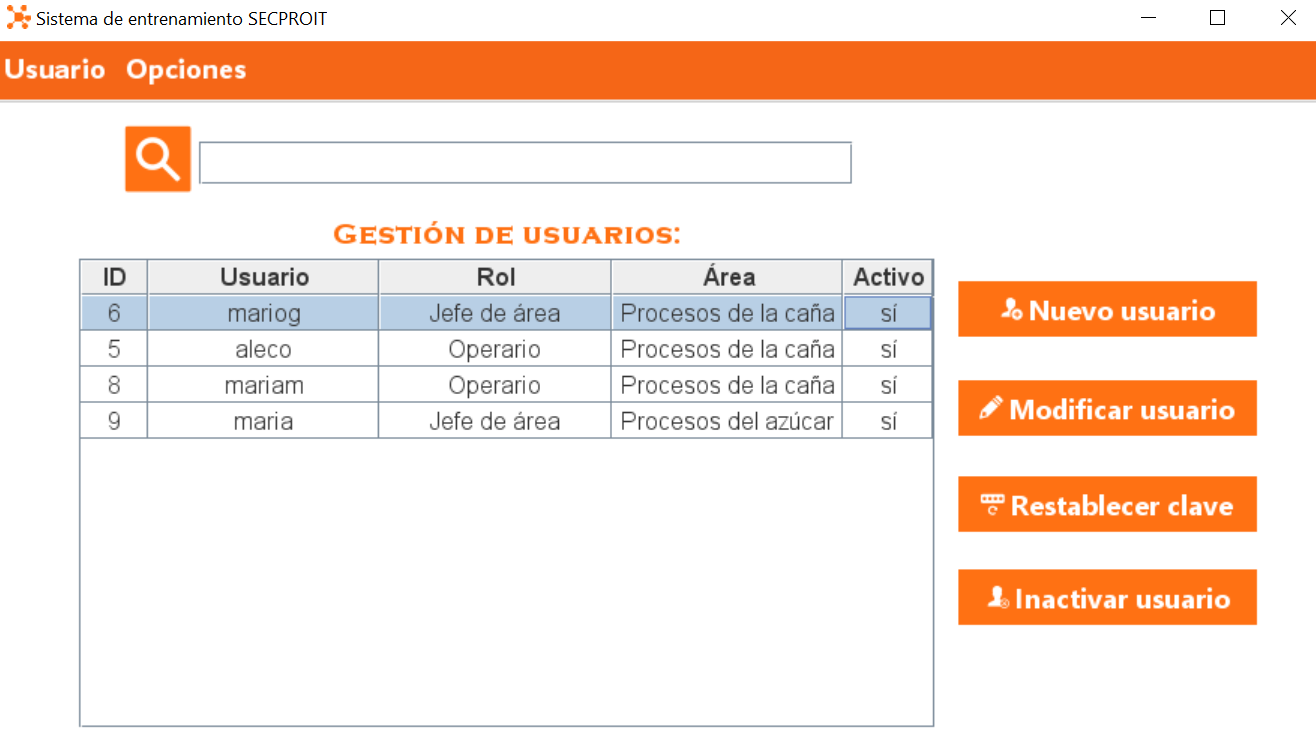
\includegraphics[width=0.9\linewidth]{imagen/anexos/usuarios.png}}
 \caption{Gestión de usuarios}
 \label{fig:gestionUss} 
\end{figure}


\section{Configuración y entrenamiento}
\begin{figure}[H]
\centering
 \frame{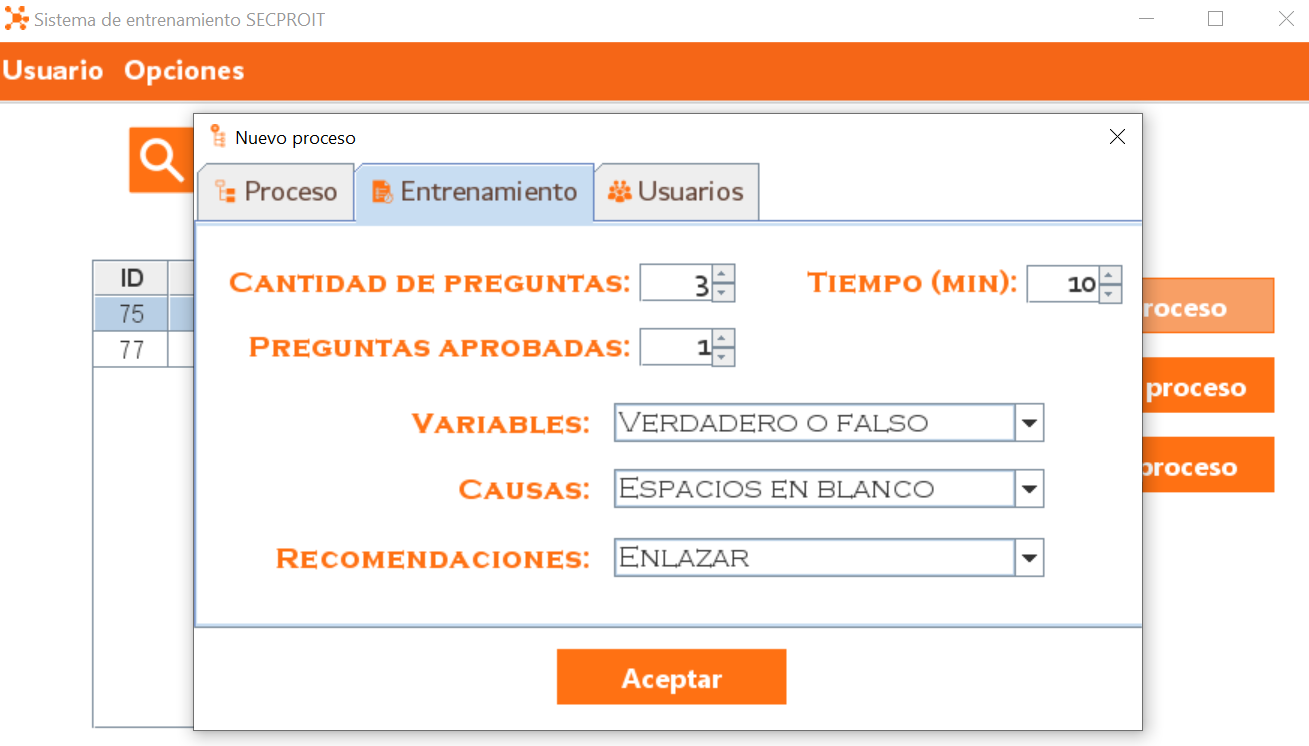
\includegraphics[width=0.9\linewidth]{imagen/anexos/nuevaConf.png}}
 \caption{Configuración de entrenamiento de un proceso}
 \label{fig:confEn} 
\end{figure}

\begin{figure}[H]
\centering
 \frame{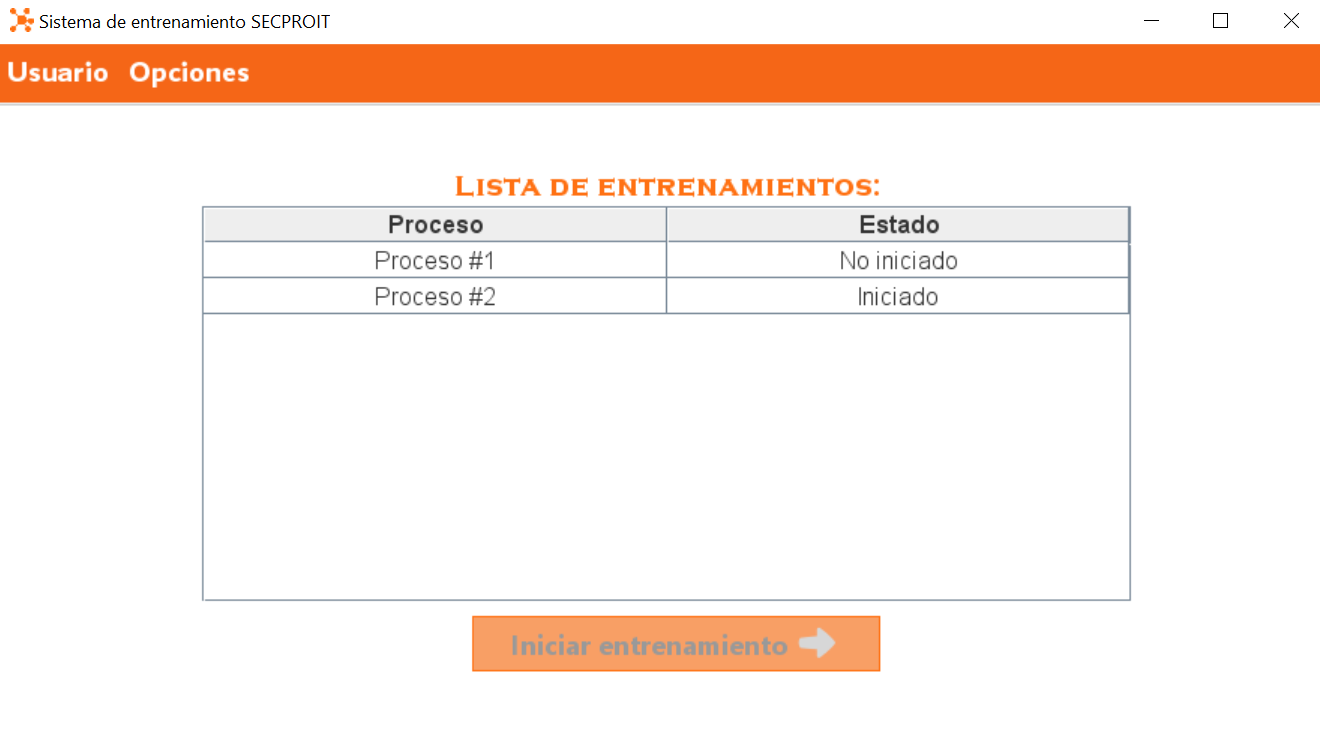
\includegraphics[width=0.9\linewidth]{imagen/anexos/listadeentrenamiento.png}}
 \caption{Listado de entrenamientos}
 \label{fig:entrenamientos} 
\end{figure}

\begin{figure}[H]
\centering
 \frame{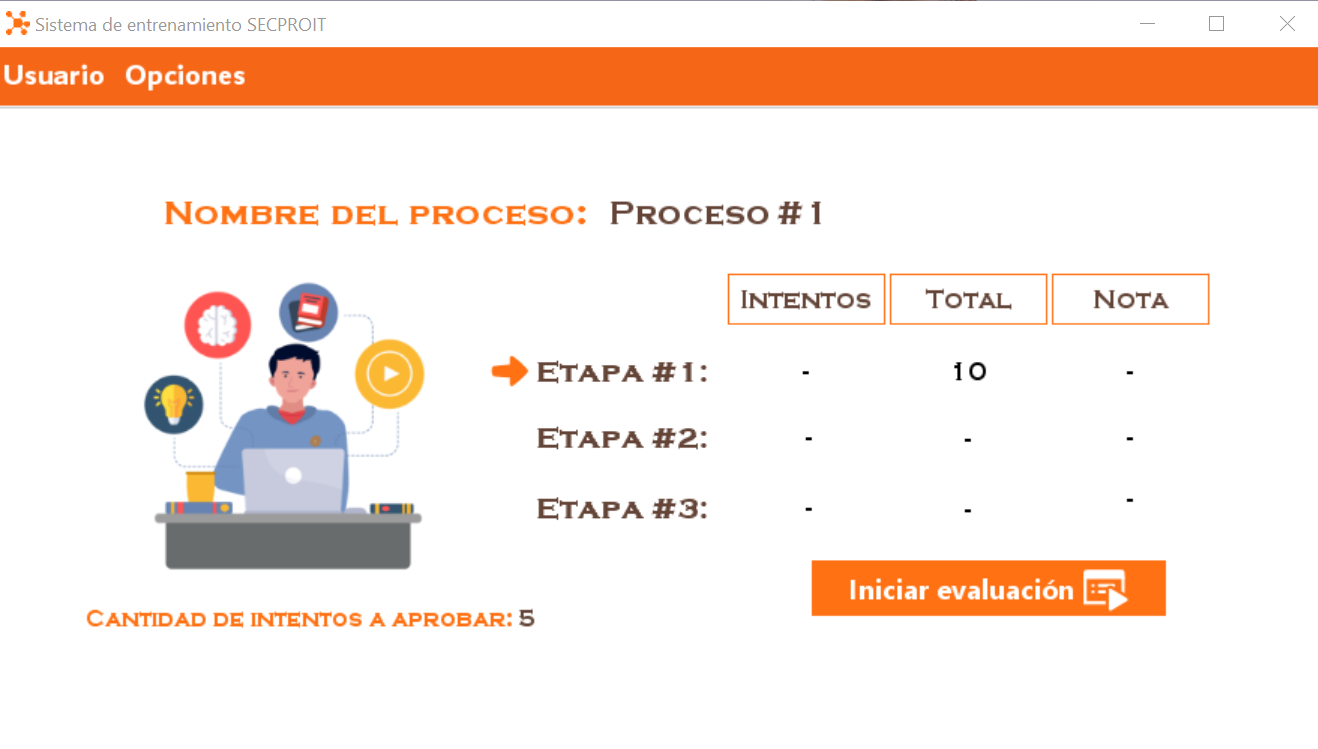
\includegraphics[width=0.9\linewidth]{imagen/anexos/eniniciado.png}}
 \caption{Entrenamiento no iniciado}
 \label{fig:eniniciado} 
\end{figure}

\begin{figure}[H]
\centering
 \frame{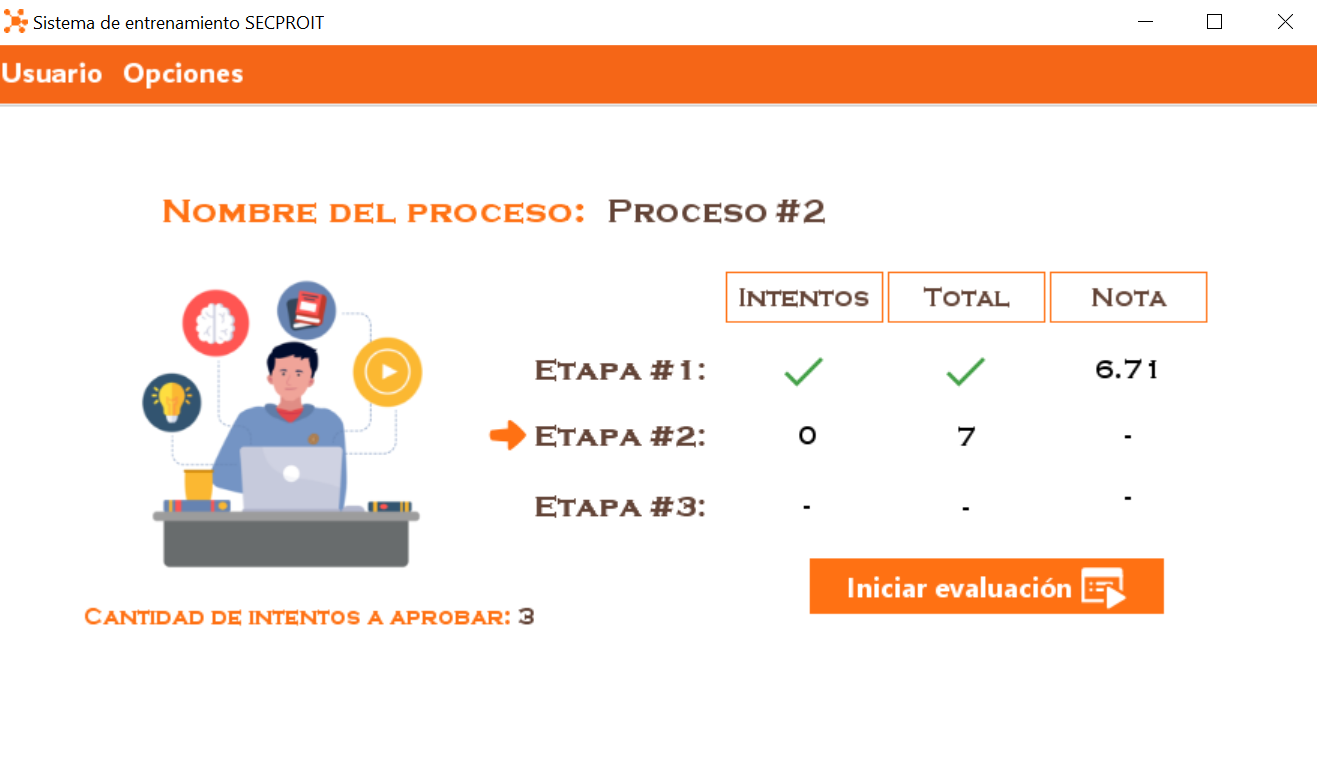
\includegraphics[width=0.9\linewidth]{imagen/anexos/einiciado.png}}
 \caption{Entrenamiento iniciado}
 \label{fig:einiciado} 
\end{figure}

\section{Tipos de preguntas en el entrenamiento}

\begin{figure}[H]
\centering
 \frame{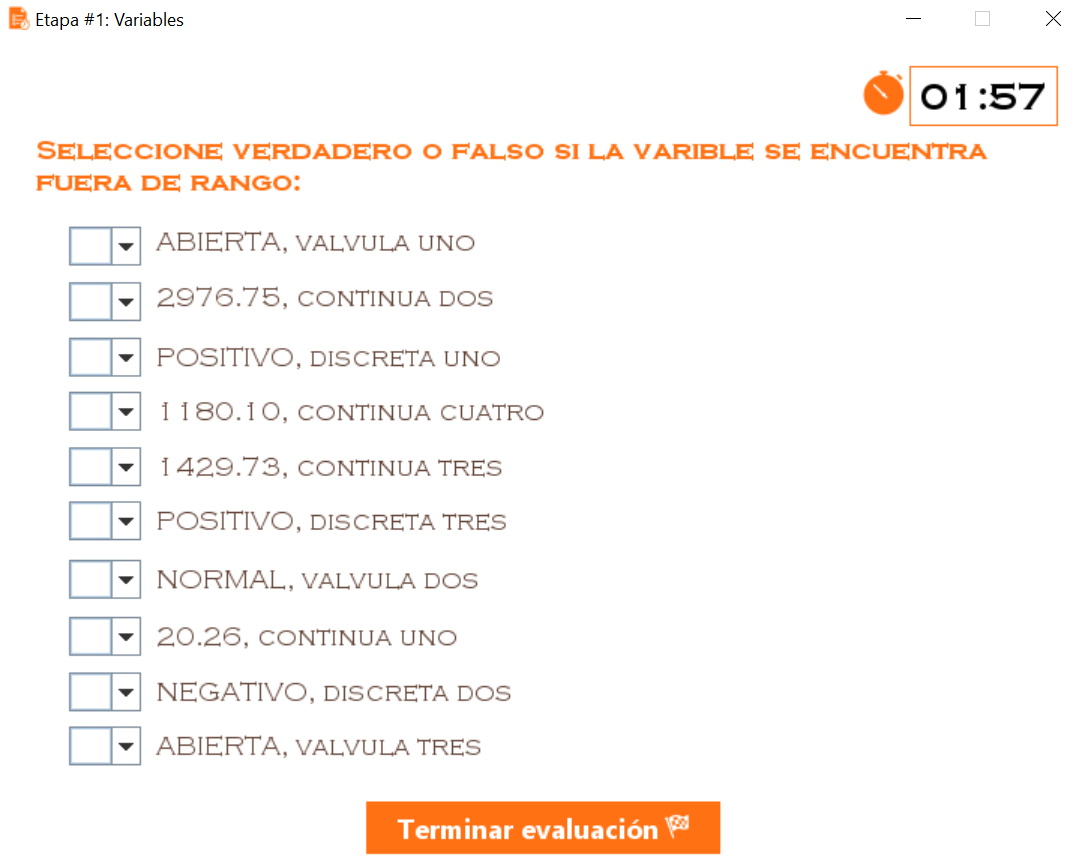
\includegraphics[width=0.7\linewidth]{imagen/anexos/pregvar.png}}
 \caption{Pregunta de verdadero o falso (en las variables)}
 \label{fig:pregvar} 
\end{figure}

\begin{figure}[H]
\centering
 \frame{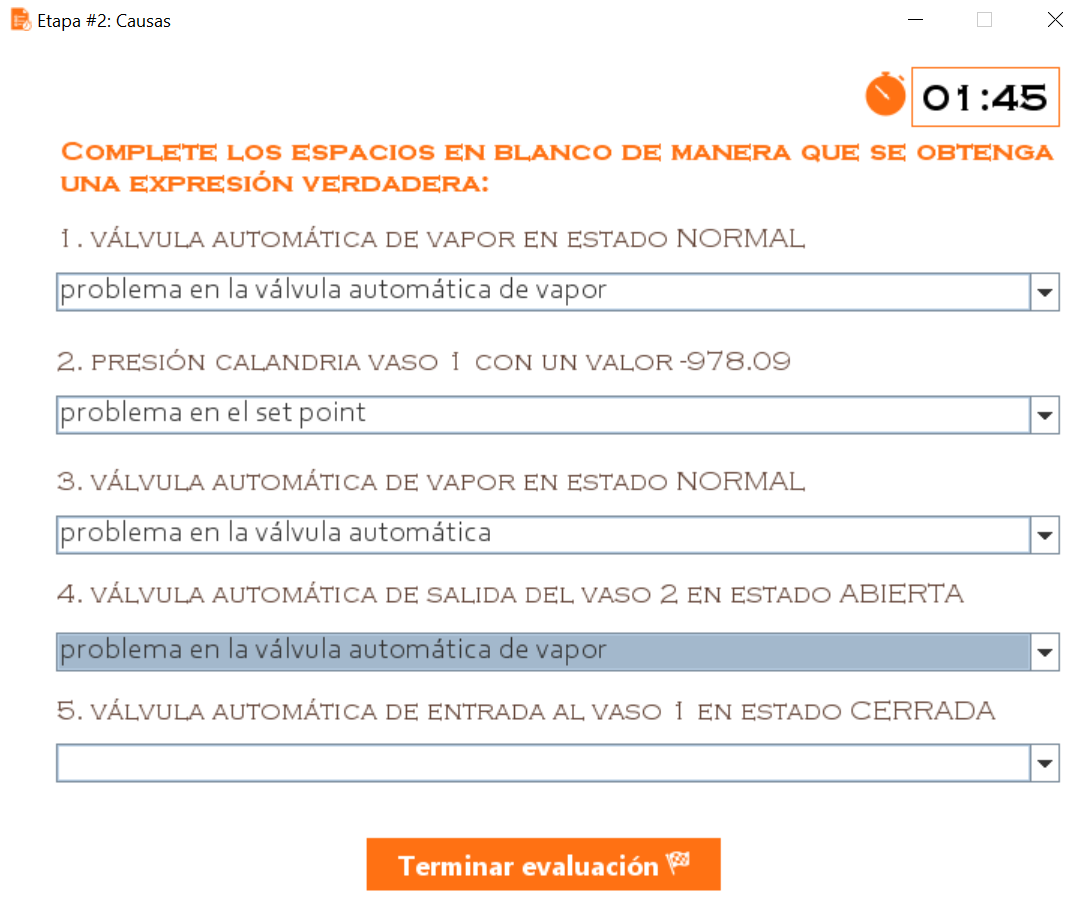
\includegraphics[width=0.7\linewidth]{imagen/anexos/pregcaus.png}}
 \caption{Pregunta de completar los espacios en blanco (en las causas)}
 \label{fig:pregcaus} 
\end{figure}


\section{Resultados obtenidos}

\begin{figure}[H]
\centering
 \frame{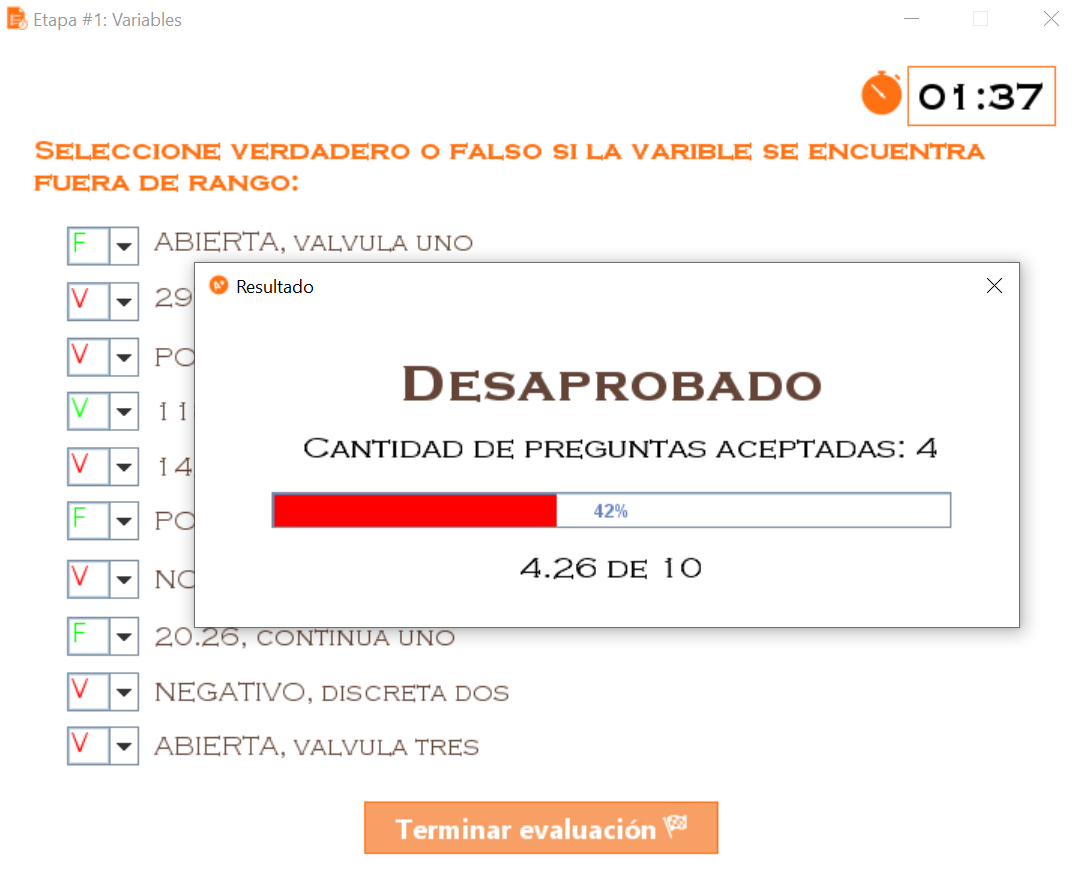
\includegraphics[width=0.9\linewidth]{imagen/anexos/notas.png}}
 \caption{Vista de los resultados obtenidos}
 \label{fig:notas} 
\end{figure}

\chapter{Pruebas funcionales del sistema}

\section{Insertar configuración de entrenamiento}
\begin{figure}[H]
\centering
 \frame{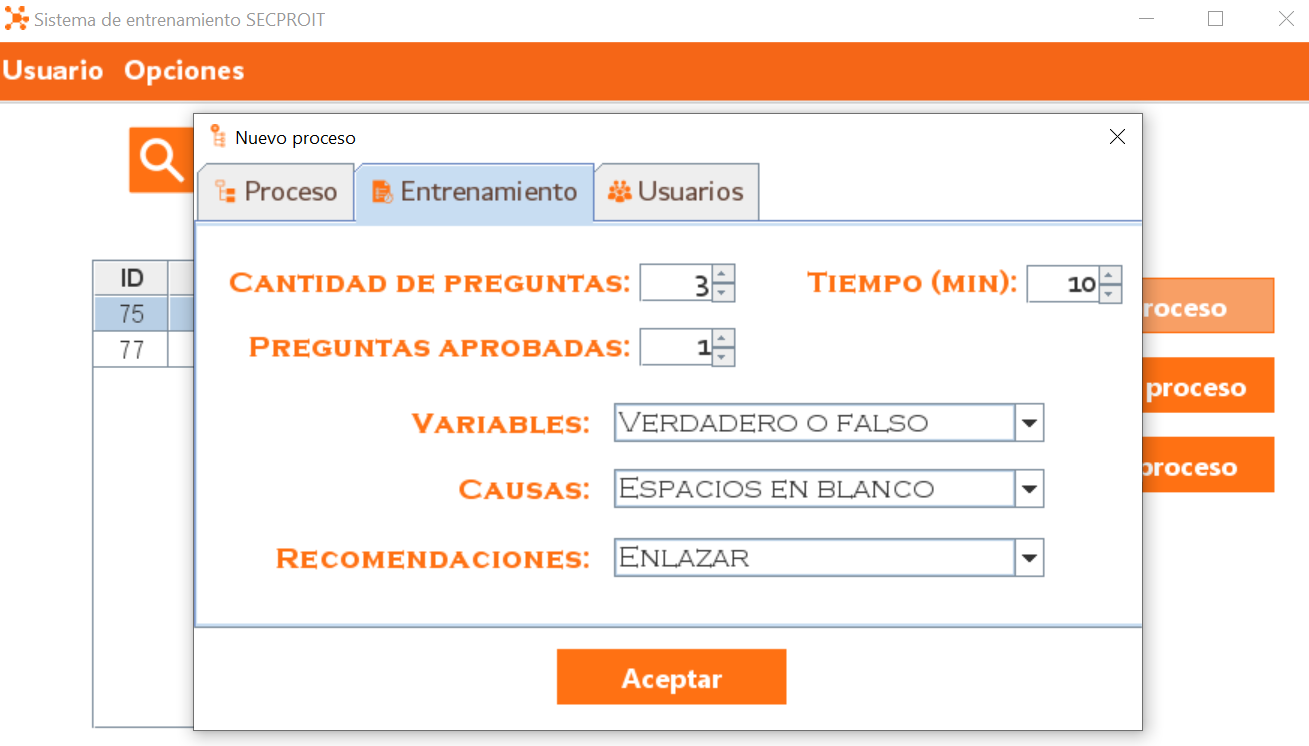
\includegraphics[width=0.9\linewidth]{imagen/anexos/nuevaConf.png}}
 \caption{Insertar configuración con campos en blanco}
 \label{fig:cb} 
\end{figure}

\begin{figure}[H]
\centering
 \frame{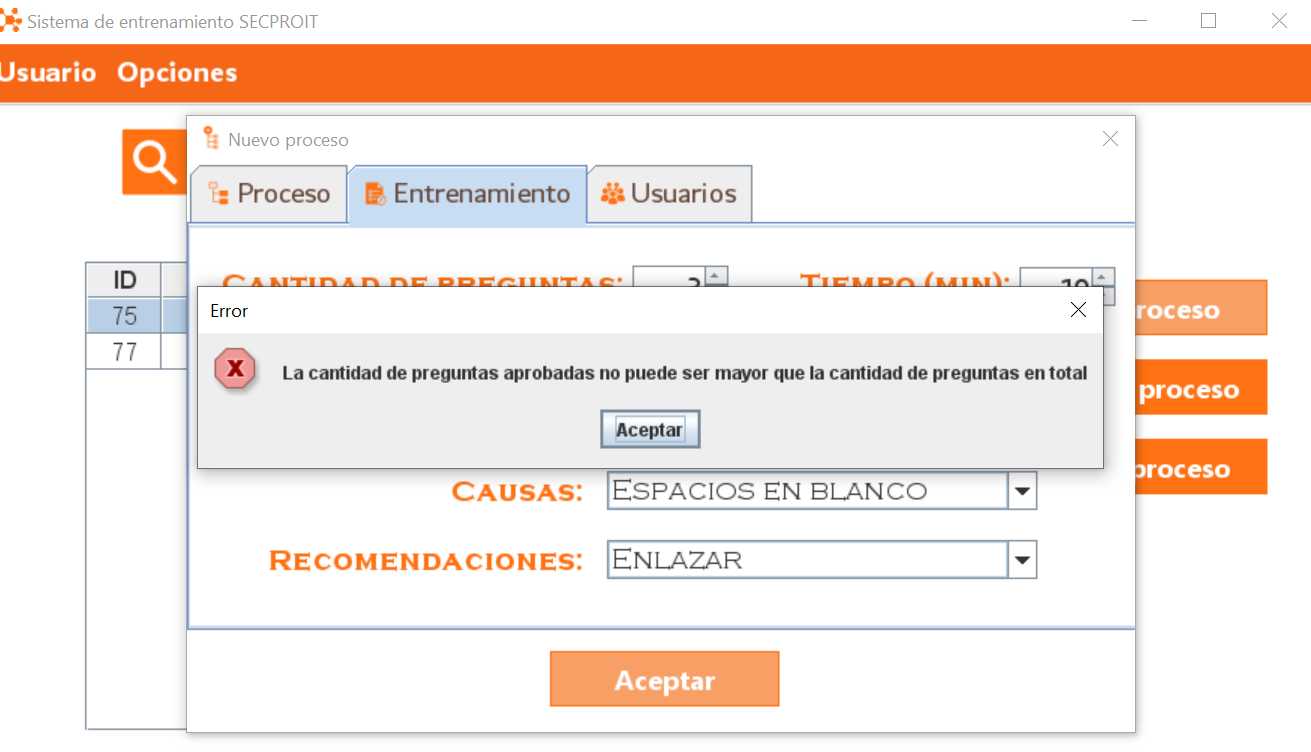
\includegraphics[width=0.9\linewidth]{imagen/anexos/errorConf.png}}
 \caption{Insertar configuración con campos incorrectos}
 \label{fig:ci} 
\end{figure}

\begin{figure}[H]
\centering
 \frame{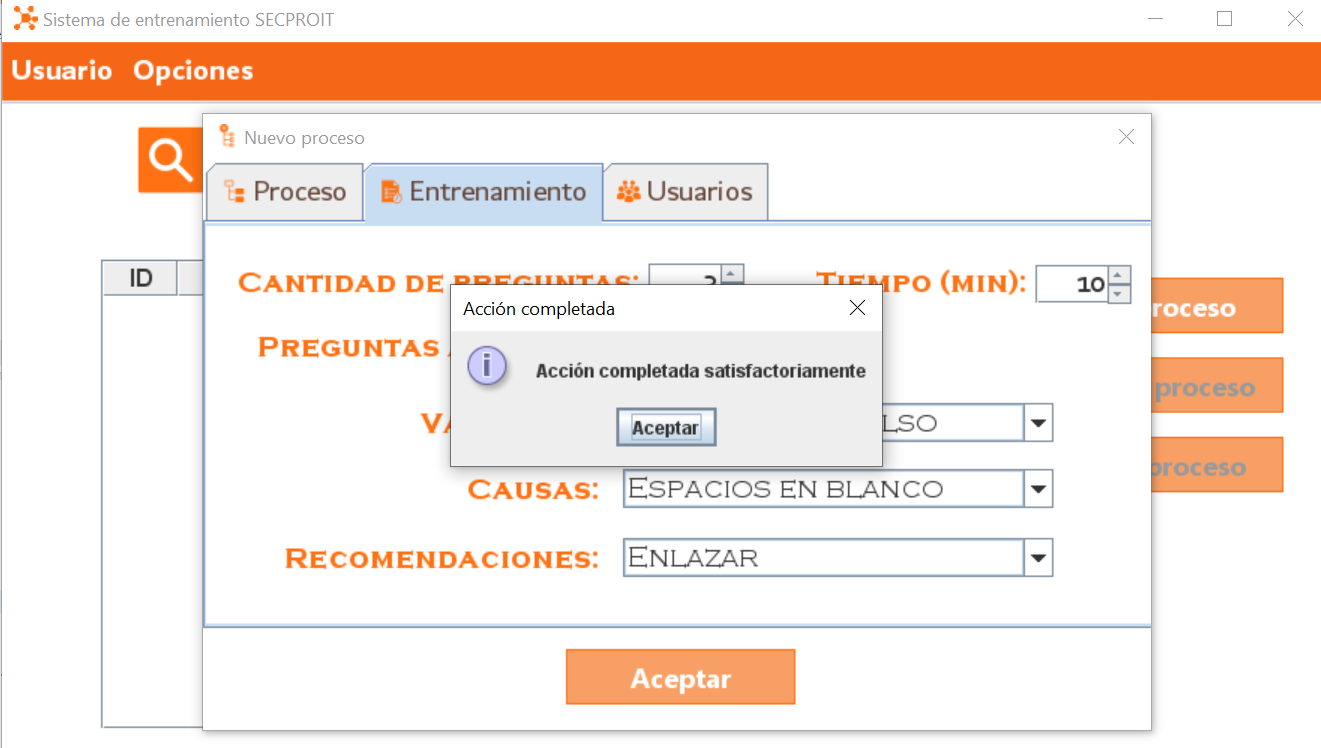
\includegraphics[width=0.9\linewidth]{imagen/anexos/guardarConf.png}}
 \caption{Insertar configuración con campos correctos}
 \label{fig:cc} 
\end{figure}

\section{Eliminar configuración de entrenamiento}
\begin{figure}[H]
\centering
 \frame{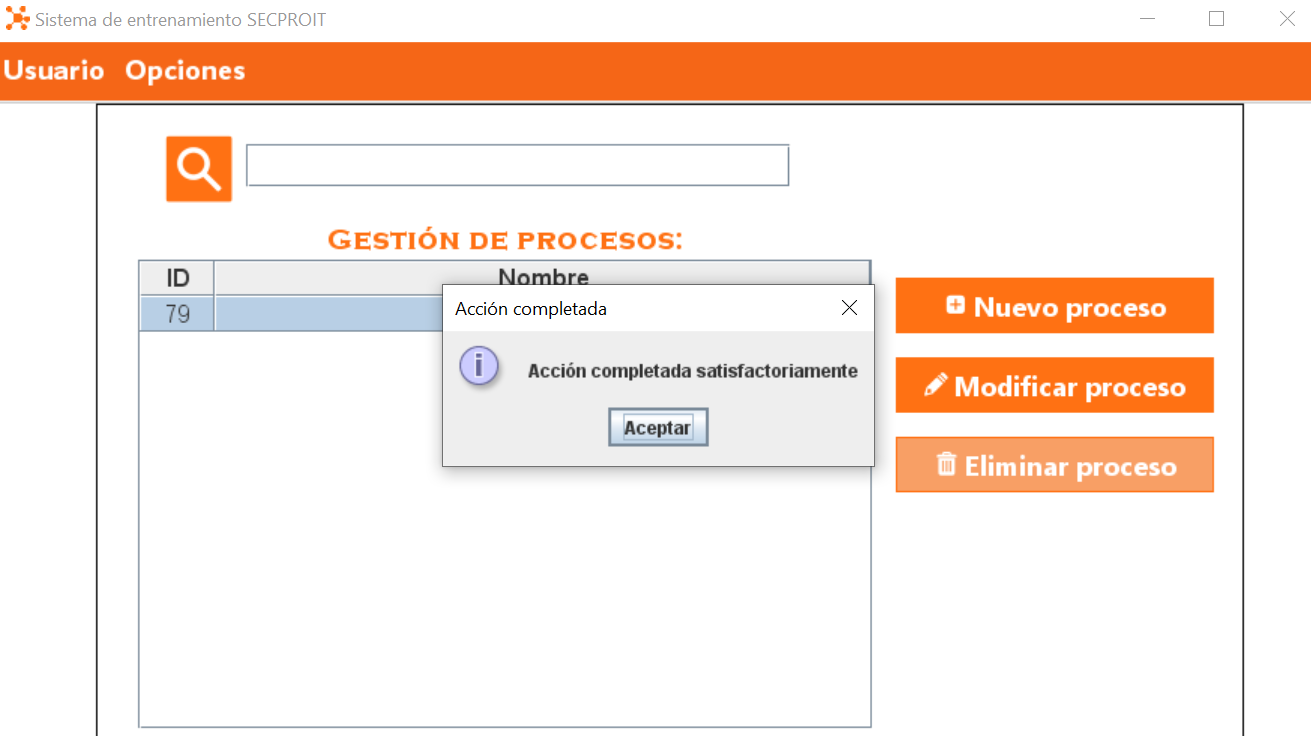
\includegraphics[width=0.9\linewidth]{imagen/anexos/eliminarConf.png}}
 \caption{Eliminar configuración de entrenamiento}
 \label{fig:ce} 
\end{figure}

\section{Entrenamiento en la etapa de las causas}
\begin{figure}[H]
\centering
 \frame{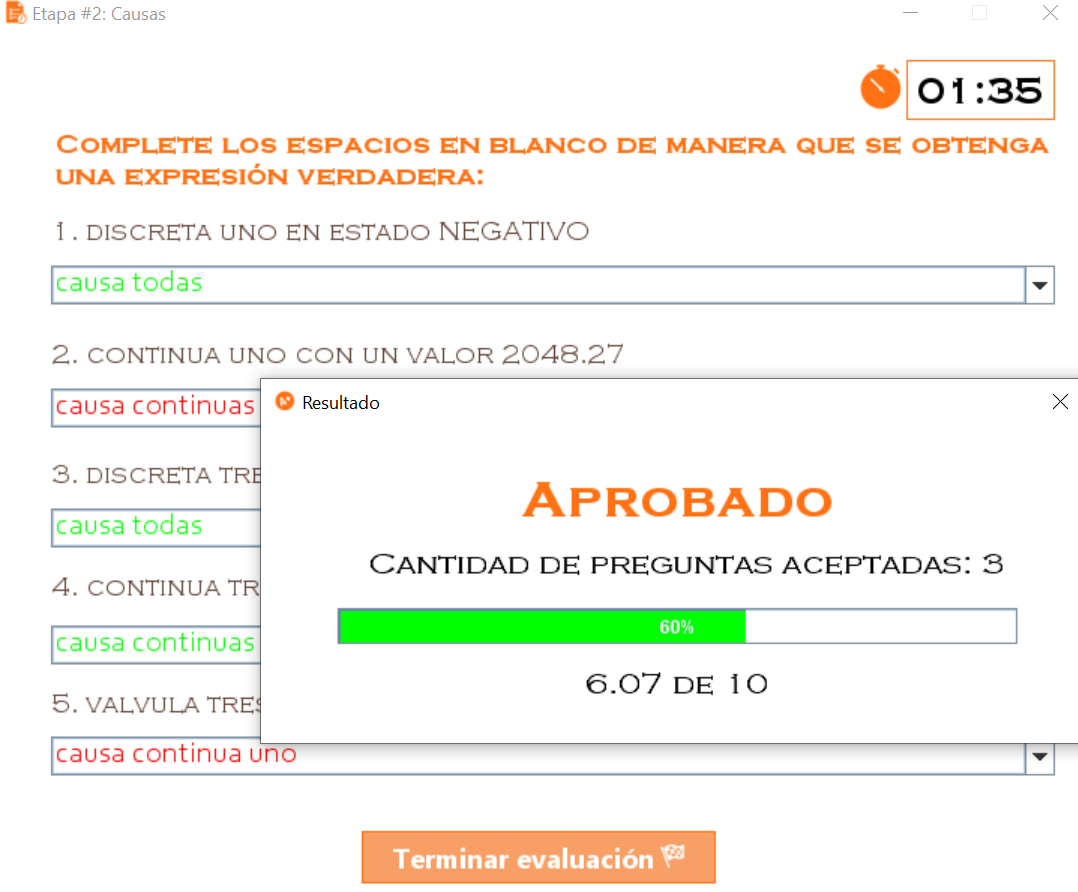
\includegraphics[width=0.7\linewidth]{imagen/anexos/causres.png}}
 \caption{Pregunta de completar los espacios en blanco}
 \label{fig:causres} 
\end{figure}

\section{Entrenamiento en la etapa de las recomendaciones}
\begin{figure}[H]
\centering
 \frame{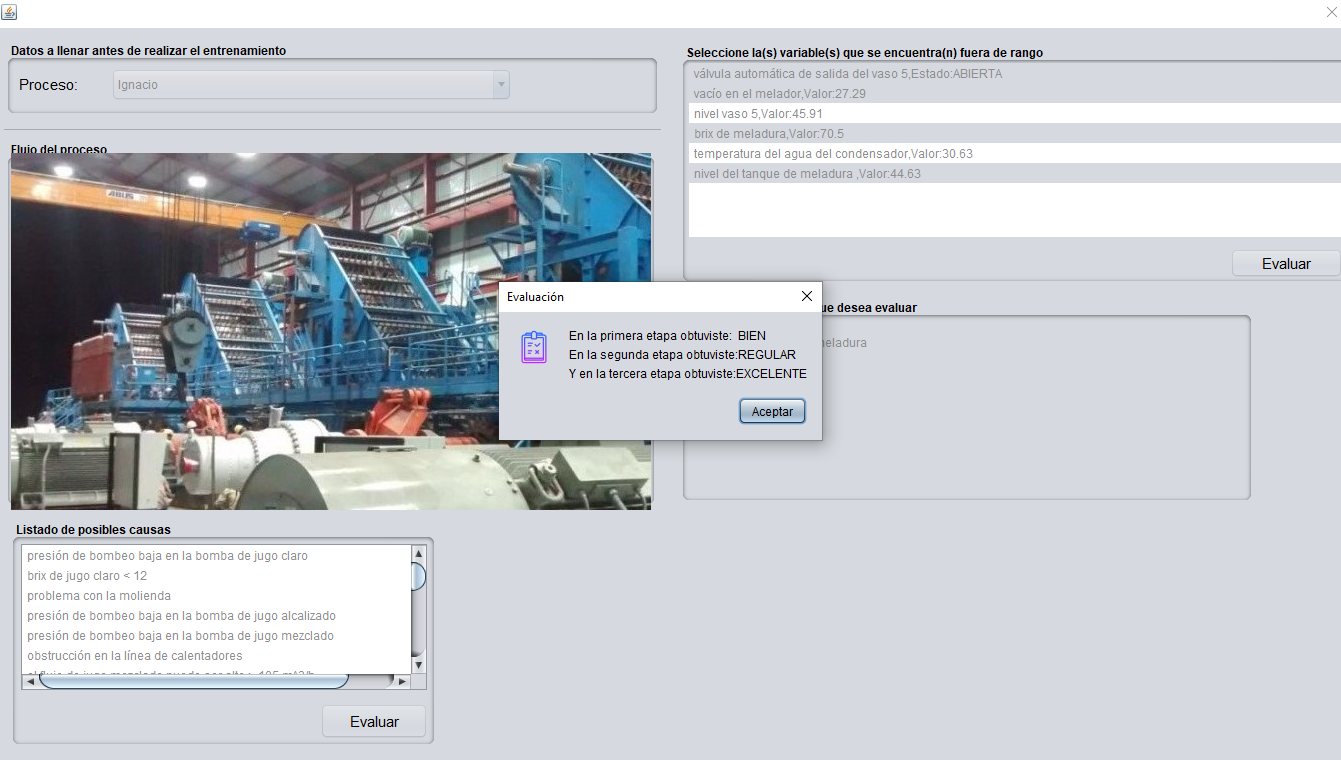
\includegraphics[width=0.9\linewidth]{imagen/anexos/errorRec.png}}
 \caption{No se evalúan las recomendaciones en el sistema SECPROIT}
 \label{fig:errorRec} 
\end{figure}